\documentclass{beamer}
\usepackage{comment}
\usepackage[utf8]{inputenc}
\usepackage{Preambles/preamble}
\usepackage{listings}
\usepackage{url}
\usepackage{graphicx}
\usepackage{amsfonts,amsmath,oldgerm,mathtools,xeCJK}
\usepackage{xcolor}
\usepackage{graphicx}
\usepackage{hyperref}
\usepackage{biblatex}
\usepackage{tikz}

\lstset{
  language=Python,
  caption={},frame=single, backgroundcolor=\color{gray!10}, basicstyle=\footnotesize, framexleftmargin=3pt, commentstyle=\color{mygreen},
  keywordstyle=\color{blue},
  stringstyle=\color{red},
  identifierstyle=\color{darkgreen},
  numbers=left,
  numberstyle=\tiny\color{gray},
  frame=single,
  rulecolor=\color{black},
  breaklines=true,
  showstringspaces=false,
  captionpos=b,
  escapeinside={(*@}{@*)}, % allows you to add LaTeX within your code
}

\addbibresource{References.bib} % Load the .bib file

\definecolor{mygreen}{rgb}{0,0.6,0}

\usetheme{sintef}

\newcommand{\testcolor}[1]{\colorbox{#1}{\textcolor{#1}{test}}~\texttt{#1}}

\usefonttheme[onlymath]{serif}

\titlebackground*{images/background.png}

\newcommand{\hrefcol}[2]{\textcolor{cyan}{\href{#1}{#2}}}

\title{Wrapping ScimBa and Feel++}
\author{Helya Amiri \and Rayen Tlili}
\date{\today}

\begin{document}
\maketitle

% -----------------------------------------------\section{Introduction}
\begin{comment}

Our goal is to streamline data exchange and empower users to leverage the combined strengths of ScimBa and Feel++ effectively.
\end{comment}

\begin{frame}[plain]
\begin{tikzpicture}[remember picture, overlay]
        \node[at=(current page.center), opacity=0.3] {
            \includegraphics[width=\paperwidth,height=\paperheight]{images/background.png}
        };
    \end{tikzpicture}
\begin{center}
    \scalebox{2}{\textbf{Main objective:}}
    \scalebox{2}{\textbf{Building an intermediary to ScimBa}} 
    \scalebox{2}{\textbf{in Feel++}}
\end{center}

\end{frame}
\begin{frame}{The main objective}
\framesubtitle{Introduction}

\begin{itemize}
    \item  \hrefcol{https://sciml.gitlabpages.inria.fr/scimba/}{Scimba :} focuses on combining machine learning with traditional scientific computing. 
    \item  \hrefcol{https://docs.feelpp.org/user/latest/index.html}{Feel++ :} is a C++ library for solving PDEs using Galerkin methods. 
\end{itemize}    

\end{frame}
% --------------------------------------------------

\begin{comment}
We will visualize and compare the results of both solvers in terms of efficiency and accuracy.

After successfully solving Poisson equations, we will extend the program's application to solve other types of PDEs.
\end{comment}

\begin{frame}{The main objectives}
\framesubtitle{Introduction}

\begin{itemize}
    \item \textbf{Create multiple results using Feel++ toolboxes.}
    \item \textbf{Using ScimBa to understand and share results}
    \item \textbf{Creating a program that can use both as solvers.}
    \item \textbf{Comparing the Results of Both Solvers}
    \item \textbf{Expand Application Scope}
\end{itemize}
\end{frame}
% --------------------------------------------------
\title{Implementation Plan}

\begin{frame}{Roadmap}
\framesubtitle{Introduction}

\begin{enumerate}
    \item Explore Feel++ and ScimBa documentation.
    \item Create a container using docker with a Feel++ base and install ScimBa within it.
    \item Solve PDEs using Feel++.
    \item Solve PDEs using ScimBa PINNs.
    \item Create a Poisson class you can call to solve using Feel++.
    \item Add ScimBa as a solver for the class by updating the Poisson2d class to handle ScimBa with parametrized f, g and add a diffusion tensor to the Poisson2d class.
    \item Compare the results of both solvers with exact solutions.
    \item Compute \( L^2\) and \( H^1 \) errors and trace their convergence for both solvers.
\end{enumerate}
\end{frame}
% --------------------------------------------------
\begin{frame}[plain]{Introduction to Feel++}
\framesubtitle{Feel++}
\begin{tikzpicture}[remember picture, overlay]
        \node[at=(current page.center), opacity=0.3] {
            \includegraphics[width=\paperwidth,height=\paperheight]{images/background.png}
        };
    \end{tikzpicture}
\begin{center}
    \scalebox{3}{\textbf{Introduction to Feel++}}
\end{center}

\end{frame}
% ------------------------------------------------\section{Feel++}

\begin{frame}{Getting familiar with Feel++}
\framesubtitle{Feel++}

\begin{itemize}
    \item Library for solving PDEs
    \item Toolboxes for math and physics-based problems
    \item Coefficient Form PDEs toolbox (CFPDE)
\end{itemize} 
\end{frame}


% --------------------------------------------------
\begin{frame}{Exploring Feel++ Toolboxes}
\framesubtitle{Feel++}

    \begin{figure}
        \centering
        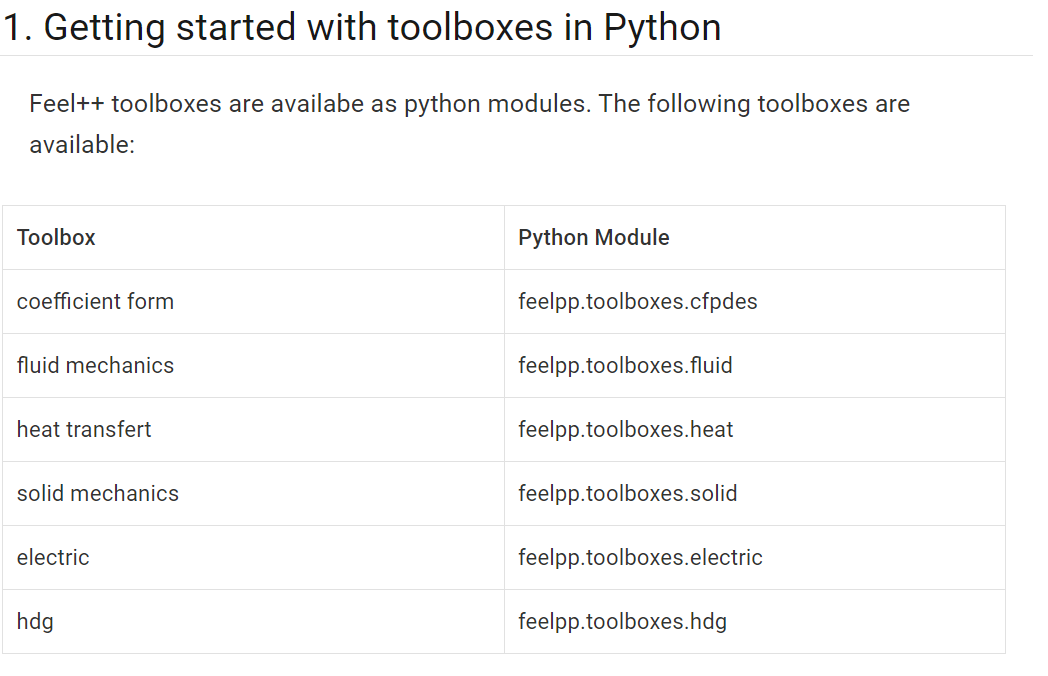
\includegraphics[width=0.7\textwidth]{images/pyfeelpptoolboxes.png}
    \end{figure}
\end{frame}
% --------------------------------------------------

\begin{frame}{CFPDE}
\framesubtitle{Feel++}
The Coefficient Form PDEs toolbox:

\begin{figure}
        \centering
        \includegraphics[width=0.7\textwidth]{images/cfpdee.png}
\end{figure}

\end{frame}
% --------------------------------------------------

\begin{comment}


ScimBa offers a Python library that merges machine learning with scientific computing



Neural Networks: MLP, RBF, and Fourier networks.
Sampling: Uniform methods for PINNs and complex geometries.
Trainers: Specific to each PDE type.
Neural Galerkin: Applies to time PDEs.
\end{comment}
\begin{frame}[plain]
\begin{tikzpicture}[remember picture, overlay]
        \node[at=(current page.center), opacity=0.3] {
            \includegraphics[width=\paperwidth,height=\paperheight]{images/background.png}
        };
    \end{tikzpicture}
\begin{center}
    \scalebox{3}{\textbf{Introduction to ScimBa}}
\end{center}

\end{frame}
%\section{ScimBa}

\begin{frame}{Getting familiar with ScimBa}
\framesubtitle{ScimBa}

ScimBa:

    \begin{itemize}
        \item Python library
        \item Merges machine learning with scientific computing
        \item Varying SciML (Scientific Machine Learning) methods for varying PDE problem
        \item Tools to build hybrid numerical methods
    \end{itemize}
\end{frame}

\begin{comment}
     PINNs integrate PDEs into neural networks by creating a loss function that penalizes errors in fitting data and violating physical laws.
\end{comment}


\begin{frame}{Getting familiar with ScimBa (PINNs)}
\framesubtitle{ScimBa}

We began utilizing examples from the ScimBa repository that employ Physics-Informed Neural Networks (PINNs).

    \vfill
    \footnotesize{\scriptsize{Schiassi, Enrico; Furfaro, Roberto; Leake, Carl; De Florio, Mario; Johnston, Hunter; Mortari, Daniele (October 2021). "Extreme theory of functional connections: A fast physics-informed neural network method for solving ordinary and partial differential equations}}
     \footnote{\tiny{Source: \url{https://sciml.gitlabpages.inria.fr/scimba/_autosummary/scimba.pinns.html#module-scimba.pinns}}}
\end{frame}




\begin{frame}[fragile]{Using ScimBa to solve a Laplacian problem in 2D}
\framesubtitle{ScimBa}
Solving the Poisson equation on a unit square domain:

\begin{lstlisting}
from lap2D_pinns import Run_laplacian2D, Poisson_2D
from scimba.equations import domain

# Define a square domain
xdomain = domain.SpaceDomain(2, domain.SquareDomain(2, [[0.0, 1.0], 
                                                    [0.0, 1.0]]))

# Create an instance of the Poisson problem
pde = Poisson_2D(xdomain)

# Run the training
Run_laplacian2D(pde)

\end{lstlisting}


\end{frame}



\begin{comment}
     The class Poisson 2D is a subclass of a predefined "pde" class that defines a problem given a specific domain.
\end{comment}


\begin{frame}[fragile]{The Poisson2D class}
\framesubtitle{ScimBa}

The parameter domain is carefully defined, to enforce specific boundary conditions or ensure solution stability.
\begin{lstlisting}
class Poisson_2D(pdes.AbstractPDEx):
    def __init__(self, space_domain):
        super().__init__(
            nb_unknowns=1,
            space_domain=space_domain,
            nb_parameters=1,
            parameter_domain=[[0.50000, 0.500001]],
        )

\end{lstlisting}

\end{frame}

\begin{comment}
The Run laplacian2D function handles everything from preparing and training a neural network to solving the Laplacian PDE using PINN. 
\end{comment}

\begin{frame}[fragile]{The Runlaplacian2D function }
\framesubtitle{ScimBa}

The Run laplacian2D covers data sampling, network setup, loss calculation, and optimization.
\begin{lstlisting}

def Run_laplacian2D(pde, bc_loss_bool=False, w_bc=0, w_res=1.0):
    x_sampler = sampling_pde.XSampler(pde=pde)
    mu_sampler = sampling_parameters.MuSampler(
        sampler=uniform_sampling.UniformSampling, model=pde
    )
    sampler = sampling_pde.PdeXCartesianSampler(x_sampler, mu_sampler)

\end{lstlisting}

\end{frame}
\begin{frame}[fragile]{Training}
\framesubtitle{ScimBa}
\begin{itemize}
    \item If \texttt{new training = False}, it suggests that you might want to continue using a previously trained and saved model without starting the training from scratch.
    \item If \texttt{new training = True}, it indicates that you want to start fresh, ignoring any previously saved models.
\end{itemize}
\begin{lstlisting}

new_training = False
#new_training = True
if new_training:
    (
        Path.cwd()
        / Path(training_x.TrainerPINNSpace.FOLDER_FOR_SAVED_NETWORKS)
        / file_name
    ).unlink(missing_ok=True)
    
\end{lstlisting}

\end{frame}

\begin{frame}[plain]
\begin{tikzpicture}[remember picture, overlay]
        \node[at=(current page.center), opacity=0.3] {
            \includegraphics[width=\paperwidth,height=\paperheight]{images/background.png}
        };
    \end{tikzpicture}
\begin{center}
    \scalebox{3}{\textbf{Setting up the Container}}
\end{center}

\end{frame}
% --------------------------------------------------\section{Docker Setup}
\begin{comment}
    
     Run the project on any platform supporting Docker
     Avoid conflicts with other software on the host system.
     Recreate the exact same environment whenever needed.
     Package all dependencies within the Docker image.
     
\end{comment}
\begin{frame}{Why use Docker?}
\framesubtitle{Docker}
    Creating a Docker container and image for the project offers these key advantages:
    \begin{enumerate}
        \item \textbf{Portability} 
        \item \textbf{Isolation} 
        \item \textbf{Reproducibility} 
        \item \textbf{Dependency Management} 
    \end{enumerate}
\end{frame}
% --------------------------------------------------
\begin{comment}
     This Dockerfile creates a docker image with Feel++ as a base and installs the dependencies and libraries needed to run ScimBa in that environment.

    
     
\end{comment}


\begin{frame}[fragile]{Creating a Docker container and image}
\framesubtitle{Docker}

Creating the Docker container

\begin{lstlisting}[language=docker,caption={Dockerfile for Feel++, Scimba, and Python libraries.},frame=single, backgroundcolor=\color{gray!10}, basicstyle=\footnotesize,rulecolor=\color{blue}, framexleftmargin=3pt, commentstyle=\color{mygreen}, keywordstyle=\color{blue}]
# Start with the Feel++ base image
FROM ghcr.io/feelpp/feelpp:jammy

# Install system dependencies
RUN apt-get update && apt-get install -y \
    git \
   xvfb

# Install Python libraries
RUN pip3 install torch xvfbwrapper pyvista plotly panel ipykernel
    matplotlib
\end{lstlisting}

\end{frame}
% --------------------------------------------------
\begin{comment}

    It copies the public ScimBa repository into the {scimba} folder and installs it.
    
    We have also built the necessary environment to run Feel++ libraries to solve a Laplacian problem and generate visuals.
    
     
\end{comment}

\begin{frame}[fragile]{Initializing the environment}
\framesubtitle{Docker}

\begin{lstlisting}[language=docker,caption={Dockerfile for Feel++, Scimba, and Python libraries.},frame=single, backgroundcolor=\color{gray!10}, basicstyle=\footnotesize,rulecolor=\color{blue}, framexleftmargin=3pt, commentstyle=\color{mygreen}, keywordstyle=\color{blue}]
# Clone the Scimba repository
RUN git clone https://gitlab.inria.fr/scimba/scimba.git 
                    /workspaces/2024-m1-scimba-feelpp/scimba

# Install Scimba and its dependencies
WORKDIR /workspaces/2024-m1-scimba-feelpp/scimba
RUN pip3 install scimba

# Copy the xvfb script into the container
COPY tools/load_xvfb.sh /usr/local/bin/load_xvfb.sh
RUN chmod +x /usr/local/bin/load_xvfb.sh

# Set the script to initialize the environment
CMD ["/usr/local/bin/load_xvfb.sh"]

\end{lstlisting}
\end{frame}
% --------------------------------------------------

\begin{frame}{Container limitations}
\framesubtitle{Docker}

    \begin{itemize}
        \item Needs access to root user
        \item Slow to build
        \item Often have to install scimba by hand inside the container
    \end{itemize}
\end{frame}

\begin{frame}[plain]
\begin{tikzpicture}[remember picture, overlay]
        \node[at=(current page.center), opacity=0.3] {
            \includegraphics[width=\paperwidth,height=\paperheight]{images/background.png}
        };
    \end{tikzpicture}
\begin{center}
    \scalebox{3}{\textbf{Methodology}}
\end{center}

\end{frame}

%\section{Methodology}


\begin{frame}[fragile]{Setting the environment}
\framesubtitle{Github}
    
Provided in the documentation are the steps necessary to set up the work environment.
\begin{figure}
    \centering
    \includegraphics[width=0.7\textwidth]{images/launch.png} 
    \label{ReadMe file in the repository}
\end{figure}

\end{frame}


\begin{frame}[fragile]{Setting the environment}
\framesubtitle{Github}
Setting the container:
\begin{figure}
    \centering
    \includegraphics[width=0.7\textwidth]{images/devco.png} 
    \label{devcontainer}
\end{figure}

\end{frame}
\begin{frame}[fragile]{Setting the environment}
\framesubtitle{Github}
Inside the '.devcontainer' folder:
\begin{lstlisting}
{
"name": "ScimBa-Feel++ 22.04",
"image": "feelpp_scimba:latest",
// Add the IDs of extensions we want installed
"extensions": [
    "ms-vscode.cpptools",
    "ms-vscode.cmake-tools",
    "josetr.cmake-language-support-vscode",
    "asciidoctor.asciidoctor-vscode",
    "ms-python.python",
    "ms-toolsai.jupyter"
]
}

\end{lstlisting}

\end{frame}




\begin{frame}[fragile]{Setting the environment}
\framesubtitle{Feel++}

Create the right environment for using the CFPDE toolbox:

\begin{lstlisting}
import sys
import feelpp
import feelpp.toolboxes.core as tb

from tools.solvers import Poisson
sys.argv = ["feelpp_app"]
e = feelpp.Environment(sys.argv,
                       opts=tb.toolboxes_options("coefficient-form-pdes", 
                       "cfpdes"),
                       config=feelpp.globalRepository('feelpp_cfpde'))

\end{lstlisting}

\end{frame}


\begin{frame}[fragile]{The Poisson class}
\title{Solving the Poisson Equation}
\framesubtitle{Feel++}

Inside that environment we want to call upon a Poisson class to solve the Poisson equation with different parameters using the CFPDE toolbox
\begin{lstlisting}
P = Poisson(dim = 2)
P(h=0.08,  rhs='-1.0-1*y*x+y*y', g='0', order=1, geofile='geo/disk.geo',
    plot='2d.png')
P(h=0.1,  rhs='-1.0-2*y*x+y*y', g='0', order=1, plot='f2.png')

P = Poisson(dim = 2)
P(h=0.1, diff='{1.0,0,0,x*y}', rhs='1', plot='d1.png')
P(h=0.1, diff='{1+x,0,0,1+y}', rhs='1', plot='d2.png')

P = Poisson(dim = 3)
P(h=0.08, diff='{1,0,0,0,x+1,0,0,0,1+x*y}', g = 'x', rhs='x*y*z', 
geofile = 'geo/cube.geo', plot='3d.png') 

\end{lstlisting}

\end{frame}



\begin{frame}[fragile]{Calling the class}
\title{Extending the Poisson Class}
\framesubtitle{Feel++ ++ ScimBa}

Adding the option to use a different solver when calling the Poisson Class:
\begin{lstlisting}
def __call__(self,
               h,                               # mesh size 
               order=1,                         # polynomial order 
               name='Potential',                # name of the variable
               rhs='8*pi*pi*sin(2*pi*x)*sin(2*pi*y)',   # right hand side
               diff='{1,0,0,1}',                # diffusion matrix
               g='0',
               geofile=None,
               plot=None,
               solver='scimba'):                # or solver='feelpp'
    """
\end{lstlisting}

\end{frame}


\begin{frame}[fragile]{Calling the class}
\framesubtitle{++Fe+el++ ++++ S++ci+m+++Ba}

\title{Solving using Feel++ and ScimBa}
Solving using Feel++ and ScimBa:
\begin{lstlisting}
P( rhs='-1.0-4*y*x+y*y', g='x', order=1, solver='feelpp')
P( rhs='-1.0-4*y*x+y*y', g='x', order=1, solver ='scimba')
\end{lstlisting}
\end{frame}

\begin{frame}[fragile]{Calling the class}
\framesubtitle{++++++++++++++++++++++++++++++++++++++}

\title{Solving using Feel++ and ScimBa}
Solving using Feel++ and ScimBa and comparing with an exact solution:
\begin{lstlisting}
P( rhs='-1-4*y*x+y*y', g='x', order=1, solver='feelpp', u_exact= u_exact)
P( rhs='-1-4*y*x+y*y', g='x', order=1, solver ='scimba', u_exact= u_exact)
\end{lstlisting}
\end{frame}


\begin{frame}[plain]
\begin{tikzpicture}[remember picture, overlay]
        \node[at=(current page.center), opacity=0.3] {
            \includegraphics[width=\paperwidth,height=\paperheight]{images/background.png}
        };
    \end{tikzpicture}
\begin{center}
    \scalebox{3}{\textbf{Results}}
\end{center}

\end{frame}
% --------------------------------------------------

\begin{frame}[fragile]{Generating visuals using Feel++}
\framesubtitle{Feel++}

Feel++ generates geometry files for either a 2D rectangle or a 3D box, compatible with Gmsh.
\begin{lstlisting}
def getMesh(filename,hsize=0.05,dim=2,verbose=False):
"""create mesh
Args:
    filename (str): name of the file
    hsize (float): mesh size
    dim (int): dimension of the mesh
    verbose (bool): verbose mode"""
                .
                .
                .
generateGeometry(filename=filename,dim=dim,hsize=hsize)
mesh = feelpp.load(feelpp.mesh(dim=dim,realdim=dim), filename, hsize)
return mesh
\end{lstlisting}

\end{frame}

\begin{frame}[fragile]{Generating visuals using Feel++}
\framesubtitle{Feel++}

Generated 3D geometry and mesh viewed using gmsh:
\begin{figure}
    \centering
    \includegraphics[width=0.4\textwidth]{images/results2.png} 
    \label{3D mesh}
\end{figure}
\end{frame}



\begin{frame}[fragile]{Generating visuals using Feel++}
\framesubtitle{Feel++}
 We initiate the Poisson class instance P by specifying the dimension as 2:
\begin{lstlisting}
P = Poisson(dim = 2)
P(h=0.08,  rhs='-1.0-1*y*x+y*y', g='0', order=1, plot='f4.png')
\end{lstlisting}
\vspace*{-0.15cm}

\begin{columns}
\column{0.6\textwidth}
\centering
\includegraphics[width=0.47\textwidth]{images/fpp_pde_2d.png}
\column{0.6\textwidth}
\centering
\includegraphics[width=0.5\textwidth]{images/fpp_pde_2d2.png}
\end{columns}
\end{frame}

\begin{frame}[fragile]{Generating visuals using Feel++}
\framesubtitle{Feel++}

 We initiate the Poisson class instance P by specifying the dimension as 3:
\begin{lstlisting}
P = Poisson(dim = 3)
P(h=0.08, diff='{1,0,0,0,x+1,0,0,0,1+x*y}', g = 'x', rhs='x*y*z', 
    geofile = 'geo/cube.geo', plot='3d.png')

\end{lstlisting}
\vspace*{-0.15cm}

\begin{columns}
\column{0.6\textwidth}
\centering
\includegraphics[width=0.4\textwidth]{images/fpp_pde_3d.png}
\column{0.6\textwidth}
\centering
\includegraphics[width=0.4\textwidth]{images/fpp_pde_3d2.png}
\end{columns}
\end{frame}

% --------------------------------------------------
\begin{frame}[fragile]{Generating visuals using ScimBa}
\framesubtitle{ScimBa}


We start by defining the spatial domain \texttt{xdomain} with ScimBa's SpaceDomain module, setting a two-dimensional square domain from $(0.0, 0.0)$ to $(1.0, 1.0)$.

%Then, we create a Poisson equation instance \texttt{pde} in two dimensions, specifying the right-hand side (\texttt{rhs}) and the boundary condition function.

Lastly, we run the \texttt{Run\_laplacian2D} function to solve the Poisson equation defined by \texttt{pde}.
\begin{lstlisting}
xdomain = domain.SpaceDomain(2, domain.SquareDomain(2, [[0.0, 1.0], 
                                                    [0.0, 1.0]]))    
pde = Poisson_2D(xdomain, rhs='8*pi*pi*sin(2*pi*x)*sin(2*pi*y)', g='0')
Run_laplacian2D(pde)
    
\end{lstlisting}

\end{frame}

\begin{frame}[fragile]{Generating visuals using ScimBa}
\framesubtitle{ScimBa}
\vspace*{-0.1cm}
The code snippet above produces the following visual representation:
\vspace*{-0.2cm}
\begin{figure}
    \centering
    
    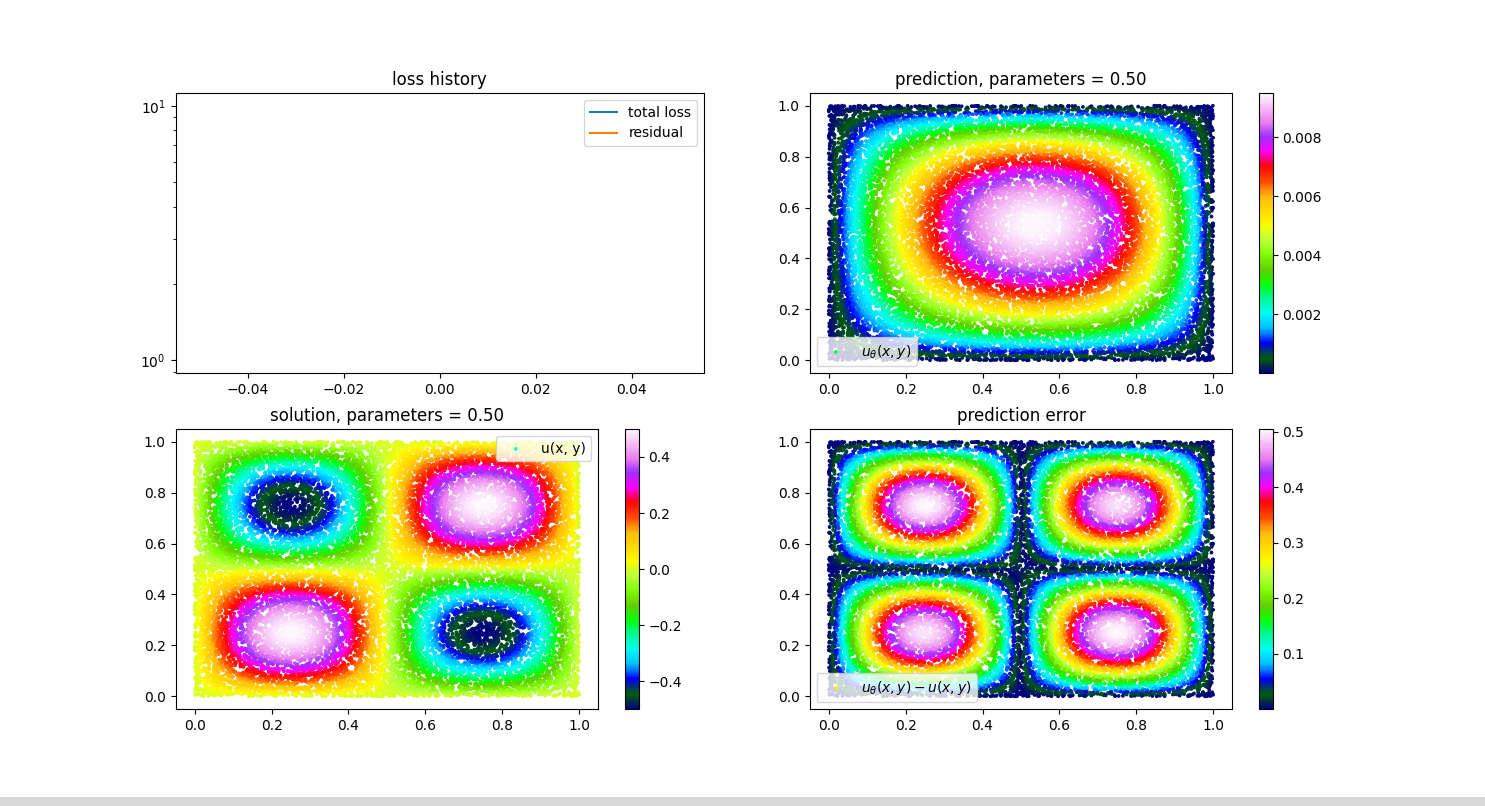
\includegraphics[width=0.85\textwidth]{images/scimbaplot1.png} 
    \label{scimba_plot}
\end{figure}
\end{frame}

\begin{frame}[fragile]{Generating visuals using ScimBa}
\framesubtitle{ScimBa}
\vspace*{-0.1cm}
The same problem with 100 epochs of training:
\vspace*{-0.2cm}
\begin{figure}
    \centering
    
    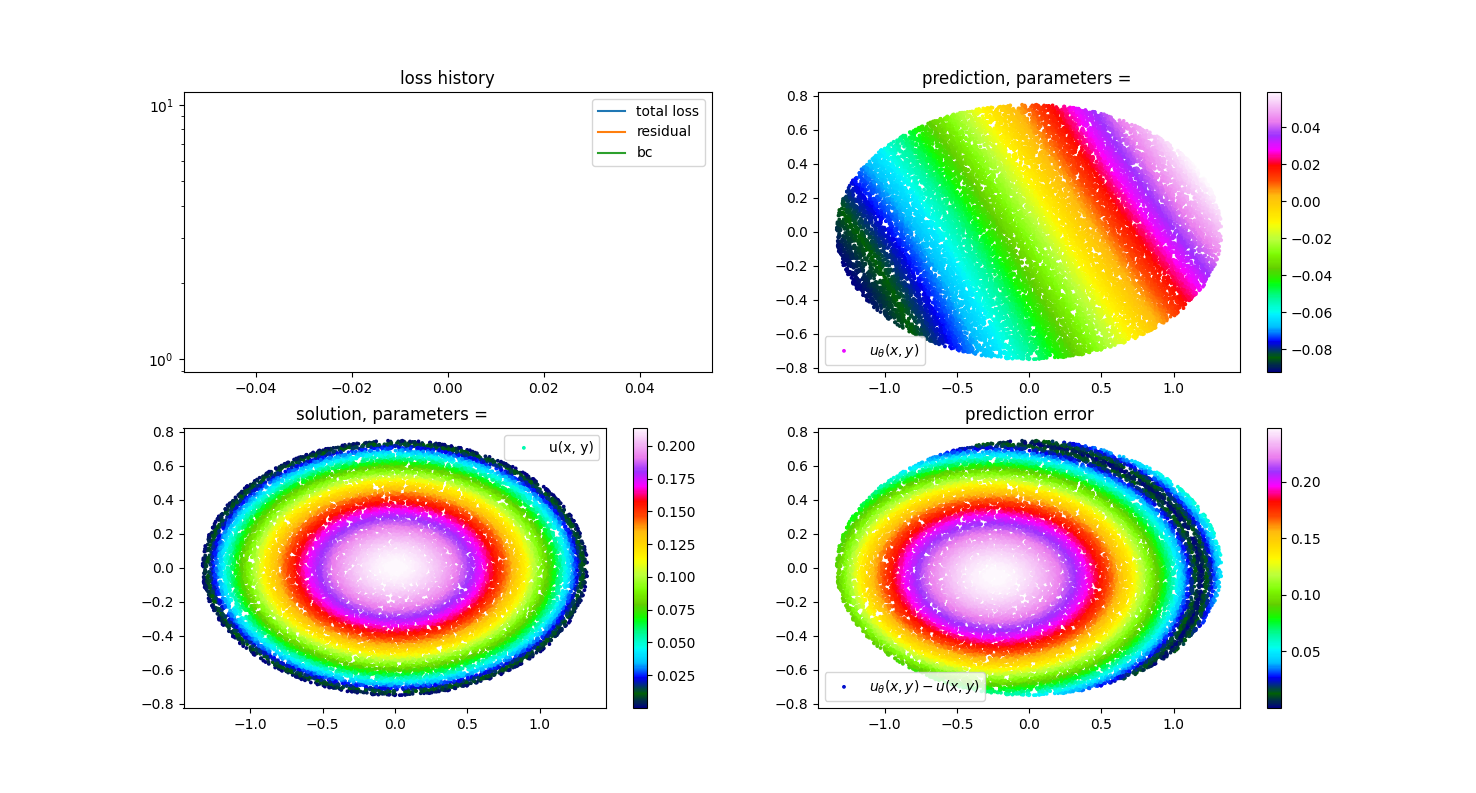
\includegraphics[width=0.85\textwidth]{images/scimbaplot3.png} 
    \label{scimba_plot}
\end{figure}
\end{frame}



\begin{frame}[fragile]{Laplacian on disk mapping}
\framesubtitle{++++++++++++}

 In this instance, we specify a two-dimensional domain utilizing a disk-based configuration with a center at $(0.0, 0.0)$ and a radius of $1.0$.

\begin{lstlisting}
xdomain = domain.SpaceDomain(2, domain.DiskBasedDomain(
                                2, center=[0.0, 0.0], radius=1.0))
    u_exact =  ' (1 - x*x - y*y)'
    rhs = '4'
    pde_disk = PoissonDisk2D(xdomain,  rhs= rhs, g= '0', u_exact=u_exact)
    Run_laplacian2D(pde_disk)
    
\end{lstlisting}
\end{frame}

\begin{frame}[fragile]{Generating visuals using ScimBa}
\framesubtitle{ScimBa}
\vspace*{-0.1cm}
The code snippet above produces the following visual representation:
\vspace*{-0.2cm}
\begin{figure}
    \centering
    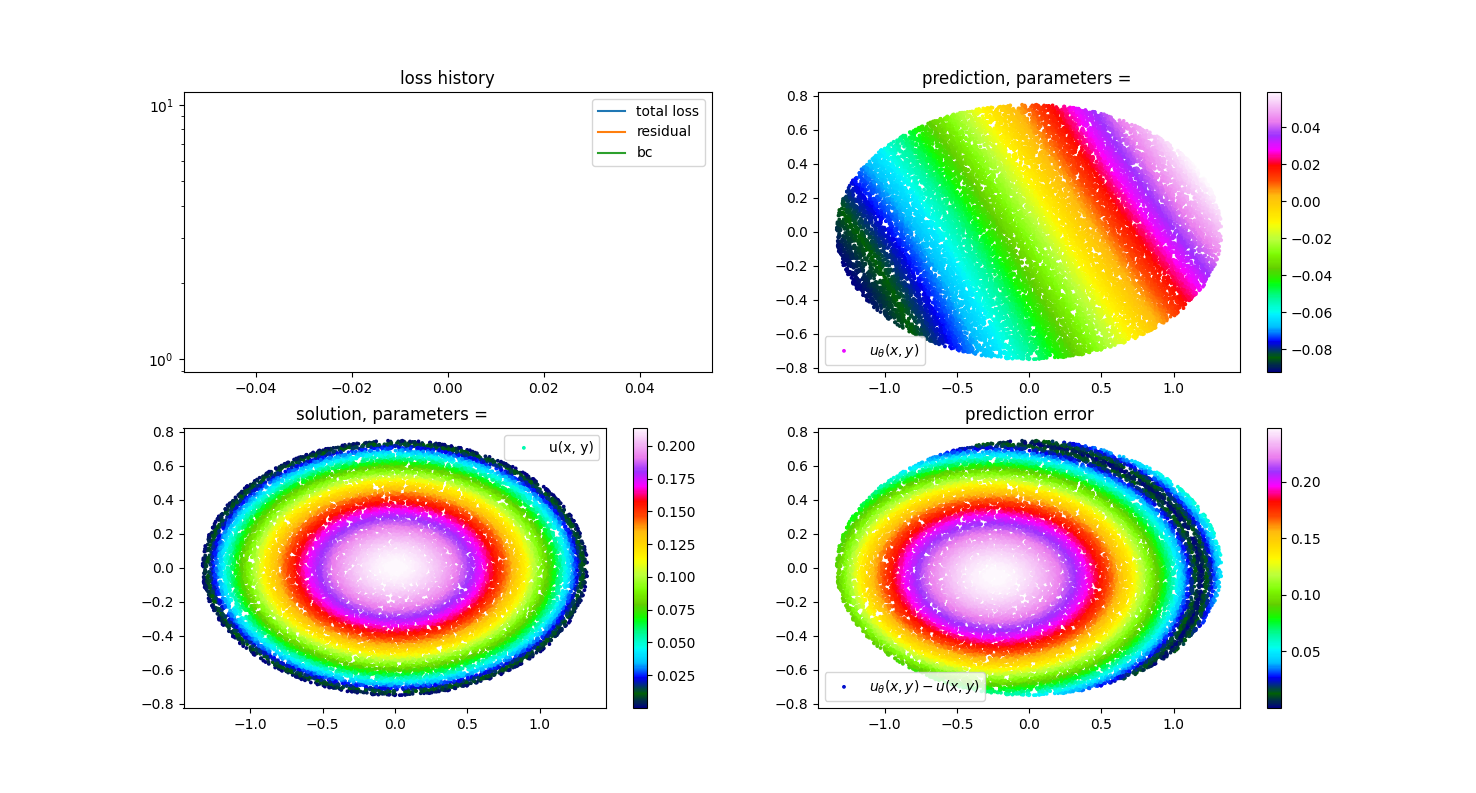
\includegraphics[width=0.85\textwidth]{images/scimbaplot3.png} 
    \label{scimba_plot}
\end{figure}
\end{frame}




% --------------------------------------------------
\begin{frame}[fragile]{Comparing the visuals for a Laplacian problem}
\framesubtitle{++++++++++++}

 This segment focuses on visualizing the solutions to the Laplacian problem on a square domain. We compare the numerical accuracy and visual fidelity of the solutions using both Feel++ and Scimba solvers.

\begin{lstlisting}
# 2D on different domains
P = Poisson(dim = 2)

# for square domain
u_exact = 'sin(2*pi*x) * sin(2*pi*y)'
rhs = '8*pi*pi*sin(2*pi*x) * sin(2*pi*y)'

P(rhs=rhs, g='0', order=1, solver='feelpp', u_exact = u_exact)
P(rhs=rhs, g='0', order=1, solver ='scimba', u_exact = u_exact)
    
\end{lstlisting}

\end{frame}



\begin{frame}[fragile]{Comparing the visuals for a Laplacian problem}
\framesubtitle{++++++++++++}


\begin{columns}
\column{0.55\textwidth}
\centering
\parbox{0.97\textwidth}{\centering \textbf{Feel++}}
\includegraphics[width=1\textwidth]{images/feel_exact.png}
\column{0.6\textwidth}
\centering
\parbox{0.97\textwidth}{\centering \textbf{ScimBa}}
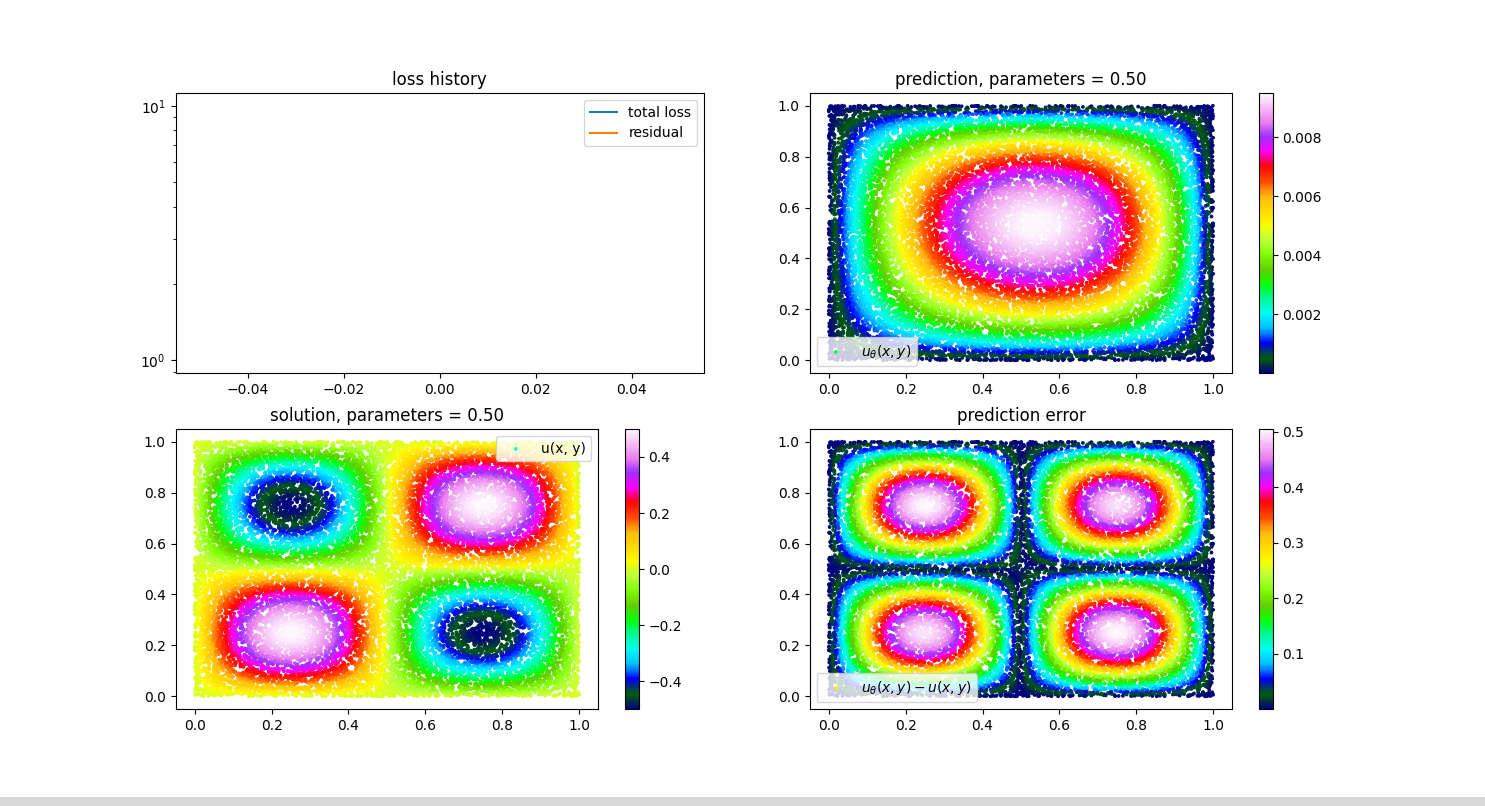
\includegraphics[width=1\textwidth]{images/scimbaplot1.png}
\end{columns}
\end{frame}


\begin{frame}[fragile]{Comparing the visuals for a Laplacian problem}
\framesubtitle{++++++++++++}

Testing the solvers' capabilities in more complex geometrical contexts.

\begin{lstlisting}

# for disk domain
u_exact =  'sin(pi*(x*x + y*y))'
rhs = '4*pi*sin(pi*(x*x + y*y)) - 4*pi*pi*(x*x + y*y)*cos(pi*(x*x + y*y))'

P(rhs=rhs, g='0', order=1, geofile='geo/disk.geo', plot='2d.png', 
    u_exact = u_exact)
P(rhs=rhs, g='0', order=1, geofile='geo/disk.geo', solver='scimba', 
    u_exact = u_exact)

    
\end{lstlisting}
\end{frame}

\begin{frame}[fragile]{Comparing the visuals for a Laplacian problem}
\framesubtitle{++++++++++++}

\begin{columns}
\column{0.55\textwidth}
\centering
\parbox{0.97\textwidth}{\centering \textbf{Feel++}}
\includegraphics[width=1\textwidth]{images/feel_disk.png}
\column{0.6\textwidth}
\centering
\parbox{0.97\textwidth}{\centering \textbf{ScimBa}}
\includegraphics[width=0.97\textwidth]{images/scimba_disk.png}
\end{columns}
\end{frame}

% --------------------------------------------------

\begin{frame}[fragile]{Error convergence rate}
\framesubtitle{++++++++++++}

\begin{lstlisting}
def runLaplacianPk(df, model, verbose=False):
    """generate the Pk case"""
    meas = dict()
    dim, order, json = model
    for h in df['h']:
        m = laplacian(hsize=h, json=json, dim=dim, verbose=verbose)
        for norm in ['L2', 'H1']:
            meas.setdefault(f'P{order}-Norm_laplace_{norm}-error', [])
            meas[f'P{order}-Norm_laplace_{norm}-error'].append(
                m.pop(f'Norm_laplace_{norm}-error'))
    df = df.assign(**meas)
    return df
\end{lstlisting}
\end{frame}


\begin{frame}[fragile]{Computing L2 and H1 errors (Computing the errors)}
\framesubtitle{++++++++++++}

This function iterates over a set of mesh sizes $h$, computes the solution using a specified computational model, and appends the L2 and H1 errors to the dataframe.
\begin{lstlisting}
df= runLaplacianPk(P, df=df, model=model, verbose=True)

\end{lstlisting}

\end{frame}

\begin{frame}[fragile]{Plotting the convergence rate}
\framesubtitle{++++++++++++}


We conduct the convergence analysis for various mesh sizes and polynomial orders. We generate and display a plot of convergence rates across mesh sizes for each polynomial order.
\begin{lstlisting}
    
df=runConvergenceAnalysis(json=laplacian_json,dim=2,verbose=True)
fig= plot_convergence(P, df,dim=2)
fig.show()

\end{lstlisting}

\end{frame}






\begin{frame}[fragile]{Tracing the convergence rate}
\framesubtitle{++++++++++++}
\vspace*{-0cm}
\begin{figure}
    \centering
    \includegraphics[width=0.7\textwidth]{images/newplot.png} 
\end{figure}
\end{frame}


% --------------------------------------------------\section{Bibliography}

\begin{frame}{Bibliography (Part 1)}
\begin{thebibliography}{14}

\setcounter{enumiv}{0}

\bibitem{coupling}
Wikipedia. (n.d.). \textit{Coupling (computer programming)}. Retrieved from \url{https://en.wikipedia.org/wiki/Coupling_(computer_programming)}

\bibitem{feelpp}
Feel++. (n.d.). \textit{Finite method course}. Retrieved from \url{https://feelpp.github.io/cours-edp/#/}

\bibitem{feelppdocs}
Feel++. (n.d.). \textit{Feel++ Documentation}. Retrieved from \url{https://docs.feelpp.org/user/latest/index.html}

\bibitem{feelppgithub}
Feel++. (n.d.). \textit{Feel++ GitHub Repository}. Retrieved from \url{https://github.com/feelpp/feelpp}

\bibitem{pyfeelpptoolboxes}
Feel++. (n.d.). \textit{Python Feel++ Toolboxes}. Retrieved from \url{https://docs.feelpp.org/user/latest/python/pyfeelpptoolboxes/index.html}

\end{thebibliography}
\end{frame}

\begin{frame}{Bibliography (Part 2)}
\begin{thebibliography}{14}

\setcounter{enumiv}{5}

\bibitem{scimba}
ScimBa. (n.d.). \textit{ScimBa Repository}. Retrieved from \url{https://gitlab.inria.fr/scimba/scimba}

\bibitem{scimba2}
SciML. (n.d.). \textit{ScimBa}. Retrieved from \url{https://sciml.gitlabpages.inria.fr/scimba/}


\bibitem{sciml}
SciML. (n.d.). \textit{Laplacian 2D Disk}. Retrieved from \url{https://sciml.gitlabpages.inria.fr/scimba/examples/laplacian2DDisk.html}

\bibitem{Quick Start with Docker}
Feel++. (n.d.). \textit{Quick Start with Docker}. Retrieved from \url{https://docs.feelpp.org/user/latest/using/docker.html}

\end{thebibliography}
\end{frame}
% --------------------------------------------------\section{Conclusion}

\begin{frame}{Conclusion}
\framesubtitle{++++++++++++}

Wrapping Feel++ with ScimBa meaningfully is a challenging task but the project was successful in certain areas yet there are still some current setbacks and potential for future work.
\end{frame}
% --------------------------------------------------
\title{}

\backmatter
\end{document}

\end{document}